\section{Work \& Energy}

In the previous chapter, we studied the accumulative effect of a force over a period of time and have seen how this gives rise to the idea of impulse and momentum. In this chapter, we consider the effect of a force over a certain displacement, and you will learn how this is related to the concept of work done and energy.

Energy is a concept central to all of physical sciences. The entire universe is made up by energy and matter. In this section we study the energy changes during various physical processes.

\subsection{work}

\begin{ilight}
	\keypoint{work done} by a force is defined as the product of the force and the displacement moved out in the direction of the force: $\boxed{W=Fs}$ \index{work}
\end{ilight}

\cmt unit for work done: $[W]=[F][s]=\text{N}\cdot\text{m}\equiv \text{J (joule)}$

if a one newton force makes an object move out by one metre, then it does work of one \keypoint{joule}

\cmt if force acts at angle $\theta$ to the displacement travelled, then: $\boxed{W=Fs\cos\theta} $

\begin{figure}[ht]
	\centering
	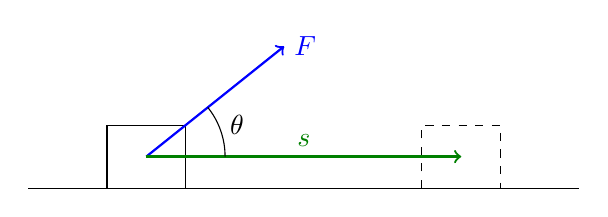
\begin{tikzpicture}
	\draw(-1,0) -- (6,0);
	\draw (0,0) rectangle (1,0.8);
	\draw[dashed] (4,0) rectangle (5,0.8);
	\draw[thick,blue,->] (0.5,0.4) --++ (1.75,1.4) node[right]{$F$};
	\draw[thick,Green,->] (0.5,0.4) -- (4.5,0.4) node[midway,above] {$s$};
	\draw (1.5,0.4) arc(0:38.66:1);
	\node at (1.65,0.8) {$\theta$};
	\end{tikzpicture}
\end{figure}

\cmt work is a \emph{scalar} quantity\footnote{Although work is defined as the product of two vectors, work carries no information about direction. This vector product is called as a \emph{scalar product} or a \emph{dot product}, which can be written explicitly as: $W = \vec{F} \cdot \vec{s} = |F||s|\cos\theta$. You might have seen this operation in the A-Level course in Mathematics.}, i.e., it has no direction


\cmt work done can be either positive or negative

resistive forces, such as friction and air drag, act in the opposite direction to motion

so work done by resistive forces is negative\footnote{You might take $\theta=180^\circ$, then $\cos\theta = -1$, giving rise to a negative work done.}, we say this is work \emph{against} resistance

the minus sign will be crucial in energy calculations in later discussions

\cmt a gas can do work to/against the surroundings

if pressure stays constant, then work by/on gas: $W = F \Delta s = p A \Delta s \RA \boxed{W_\text{gas} = p\Delta V}$

\cmt work done by a varying force\footnote{The equation $W=Fs$ is valid only if the force acting is constant.
	
Similarly, the equation $W_\text{gas} = p\Delta V$ holds for constant pressure processes only.} is found by integration or using a $F$-$s$ graph



if force varies with position, its change over small displacements is still considered small

work done over an infinitesimal displacement is therefore $\dd W = F\dd s$

integrate from initial position to final position, total work done is given by: $ \boxed{W=\int_i^f F \dd s} $

if one plots force against displacement, then $\boxed{\text{area under $F$-$s$ curve gives work done}}$

\example{A 20 N force is applied at 60$^\circ$ to the horizontal to move a 1.0 kg object at a constant speed of 2.0$\mps$ for 30 s. How much work is done by the force?}

\solc \begin{equation*}
W = Fs\cos\theta = Fvt\cos\theta = 20 \times 2.0 \times 30 \times \cos60^\circ \RA W = 600\text{ J} \teoe
\end{equation*}

\example{A piston in a gas pump has an area of 600 cm$^2$. During one stroke, the pump moves a distance of 30 cm against a constant pressure of 8000 Pa. How much work is done?}

\solc \begin{equation*}
W = p \Delta V = p A \Delta s = 8000 \times 600 \times 10^{-4} \times 30 \times 10^{-2} \RA W = 144 \text{ J} \teoe
\end{equation*}


\begin{wrapfigure}{r}{0.36\textwidth}
	\vspace*{-12pt}
	\centering
	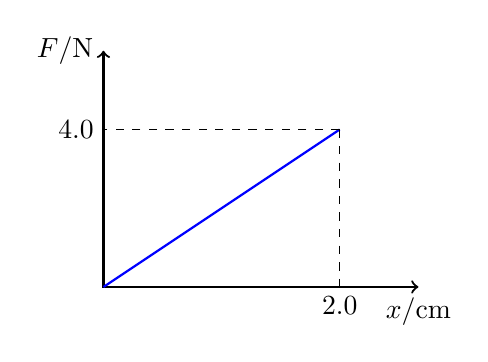
\begin{tikzpicture}
		\draw[thick,<->] (4,0) node[below]{$x$/cm} -- (0,0) -- (0,3) node[left]{$F$/N};
		\draw[thick,blue] (0,0) -- (3,2);
		\draw[dashed] (3,2) -- (3,0) node[below] {$2.0$};
		\draw[dashed] (3,2) -- (0,2) node[left] {$4.0$};
	\end{tikzpicture}
	\vspace*{-16pt}
\end{wrapfigure}

\example{When a spring is compressed by 2.0 cm, the force applied increases uniformly from zero to 4.0 N. How much work is done by this force?}

\sol $F$-$x$ graph for the force is plotted as shown

work to compress spring equals area under $F$-$x$ graph:

{
	\centering
	
	$ W = \frac{1}{2} \times 4.0 \times 2.0 \times 10^{-2} = 0.040 \text{ J} $
	
	\vspace*{-\baselineskip} \eoe
	
}



\subsection{types of energies}\label{ch-KE}

Energy is something acquired by an object that enables it to do work. A moving vehicle, water stored in a reservoir, a compressed spring, separated magnets, all of these objects can do work to other objects. In this section, we will look at various situations where work on an object causes a change in some form of energy.


\subsubsection{kinetic energy}

suppose a constant force $F$ is acting over a distance $s$, we have:
\begin{equation*}
	W=Fs \xlongequal{F=ma} mas \xlongequal{v^2 = u^2 + 2as} m \frac{v^2-u^2}{2} \RA W = \frac{1}{2}mv^2 - \frac{1}{2}mu^2
\end{equation*}

this shows work is transformed into change in some quantity associated with object's motion

this is recognised as the gain in kinetic energy of the object: $ \Delta E_k = \frac{1}{2}mv^2 - \frac{1}{2}mu^2 $

\begin{ilight}
	\keypoint{kinetic energy} (K.E.) is the energy possessed by an object due to its motion  \index{energy!kinetic}
\end{ilight}

\cmt an object of mass $m$ moving with speed $v$ has K.E.: $ \boxed{E_k = \frac{1}{2}mv^2} $

\example{Estimate the kinetic energy of a running man.}

\sol suppose the man has a mass of 75 kg and is running at $5 \mps$ (any reasonable value will do)
\begin{equation*}
	E_k = \frac{1}{2}mv^2 = \frac{1}{2}\times75\times5^2 \approx 940 \text{ J} \teoe
\end{equation*}



\subsubsection{gravitational potential energy}

\begin{wrapfigure}{r}{0.3\textwidth}
	\vspace*{-12pt}
	\centering
	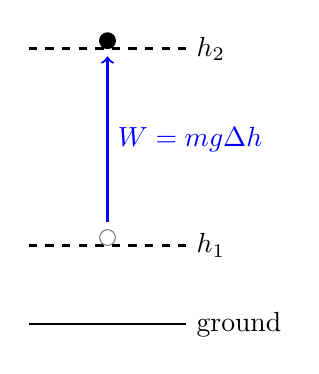
\begin{tikzpicture}
		\draw[thick,dashed] (0,1.5) --++ (2,0) node[right]{$h_1$}; 
		\draw[thick,dashed] (0,4) --++ (2,0) node[right]{$h_2$};
		\draw[fill] (1,4.1) circle (0.1);
		\draw[gray] (1,1.6) circle (0.1);
		\draw[thick,blue,->] (1,1.8) -- (1,3.9) node[midway,right]{$W=mg\Delta h$};
		\draw[thick] (0,0.5) --++ (2,0) node[right]{ground};
	\end{tikzpicture}
	\vspace*{-16pt}
\end{wrapfigure}


consider a body being slowly pulled from a height of $h_1$ to $h_2$

work done for this process is: $W = Fs = mg\Delta h = mgh_2 - mgh_1$

this shows work is transformed into change in some quantity associated with object's position

we say this is the gain in gravitational potential energy:

{
	\centering
	
	$\Delta E_p = mgh_2 - mgh_1$
	
}

\begin{ilight}
	\keypoint{gravitational potential energy} (G.P.E.) is the energy possessed by a body due to its position in a gravitational field\index{energy!gravitational potential}
\end{ilight}

\cmt a body of mass $m$ at a height of $h$ has G.P.E.: $\boxed{E_p = mgh}$

\cmt G.P.E. is a \emph{relative} quantity, only its change is important in physical processes
\footnote{The formula $E_p = mgh$ implies that we have defined G.P.E. at the ground level to be zero. But this is purely conventional. Here I would like to point out that one can freely choose any zero potential energy level as he/she wishes, but no matter what point is picked as reference, we will always agree on the quantity of physical significance, that is, the \emph{change} in G.P.E between two fixed points.}






\subsubsection{elastic potential energy}

let's now consider a spring being stretched or compressed

work is done by external forces to cause the change in shape

this becomes of the elastic energy stored in the body

\begin{ilight}
	\keypoint{elastic potential energy}, also called \keypoint{strain energy}, is the energy possessed by an elastic body due to deformation \index{energy!elastic potential}
\end{ilight}

this topic will be revisited in details in \S\ref{ch-spring-energy}

\subsubsection{other types of energies}

apart from those we have mentioned above, there are many other types of energies 

\titem \emph{electric potential energy}: energy of a charged object due to its position in an electric field

\titem \emph{chemical energy}: ability to do work due to potential energy between atoms and molecules

\titem \emph{nuclear energy}: ability to do work due to potential energy of subatomic particles in the nuclei

\titem \emph{internal energy}: sum of random kinetic and potential energies of molecules in a substance

\titem \emph{electromagnetic energy}: energy carried by light/electromagnetic waves


\subsubsection{work \& energy transformations}

from previous discussions, we have seen doing work is a way of transferring energy

for examination purposes\footnote{More rigorous discussions (which go beyond the syllabus) are given in \S\ref{ch:conservation-of-energy}.}, we can say the following:

\begin{ilight}
	the change in the total energy of an object equals the net work done by all external forces (excluding those associated with potential energies): $\boxed{W  = \Delta E} $
\end{ilight}

\example{A racing car of 800 kg starts off from rest. If the driving force is 5000 N, and the car experiences a constant resistive force of 1500 N, what is its speed after it has travelled 50 m?}

\sol gain in K.E. equals work by driving force plus \emph{negative} work against resistance
\begin{equation*}
W_\text{total} = \Delta E_k \RA Fs - fs = \frac{1}{2}mv^2 - 0 \RA (5000 - 1500)\times50 = \frac{1}{2}\times800\times v^2 \RA v\approx20.9\mps \teoe
\end{equation*}

\example{A concrete cube of side 0.50 m and density 2400 kg m$^{-3}$ is lifted 4.0 m by a crane. How much work is done?}

\sol work by crane equals gain in G.P.E. of cube
\begin{equation*}
W = \Delta E_p \RA W = mg\Delta h = \rho V g \Delta h = 2400 \times 0.50^3 \times 9.81 \times 4.0 \approx 1.18\times10^4 \text{ J} \teoe
\end{equation*}


\subsection{conservation of energy}\label{ch:conservation-of-energy}

\subsubsection{work-energy theorem ($\star$)}

more generally, net work done due to several forces $F_1$, $F_2$, $\dots$, acting on an object is
\begin{equation*}
W_\text{total} = \sum W_i = \sum \left(\int_i^f F_i \dd s\right) = \int_i^f \left(\sum F_i \right)\dd s = \int_i^f F_\text{net} \dd s = \int_i^f ma \dd s
\end{equation*}

recall in kinematics, $a=\frac{\dd v}{\dd t}$ and $\dd s = v \dd t$, so we have
\begin{equation*}
W_\text{total} = \int_i^f m \frac{\dd v}{\dd t} v \dd t = \int_i^f m v \dd v
\end{equation*}

we are integrating over velocity from initial value $u$ to final value $v$, so we find
\begin{equation*}
W_\text{total} = \int_i^f m v \dd v = \frac{1}{2}mv^2 \Big|_u^v = \frac{1}{2}mv^2 - \frac{1}{2}mu^2
\end{equation*}

identify kinetic energy $E_k = \frac{1}{2}mv^2$, now we come to the \keypoint{work-energy theorem}  \index{work-energy theorem}

\begin{ilight}
	the net work done on a body equals the change in the body's kinetic energy: $\boxed{W_\text{total} = \Delta E_k}$
\end{ilight}



\subsubsection{conservative forces \& potential energy ($\star$)}


if work by a force does not depend on which specific path is taken, this force is \keypoint{conservative}

put differently, when an object is moved from one place to another under a conservative force, work done depends on initial and final positions only

we can split $W_\text{total}$ into two parts: contributions from conservative and non-conservative forces

for conservative part, let's define: $\Delta E_p = - W_{c} = - \int_i^f F_c \dd s $

this means work by conservative forces can be interpreted as change in its \keypoint{potential energy}

let's call the sum of an object's kinetic and potential energy its \keypoint{mechanical energy}: $E_m = E_k + E_p$

work-energy theorem can then be rewritten: $\Delta E_k = W_\text{total} = W_\text{c} + W_\text{nc} = -\Delta E_p + W_\text{nc}$

rearrange we have: $W_\text{nc} = \Delta E_k + \Delta E_p \RA  \boxed{W_\text{nc} = \Delta E_m}$

\begin{ilight}
	the change in mechanical energy equals the net work done by all non-conservative forces
\end{ilight}


\newpage

\subsubsection*{gravitational potential energy revisited ($\star$)}

\begin{wrapfigure}{R}{0.32\textwidth}
	\vspace{-54pt}
	\begin{center}
		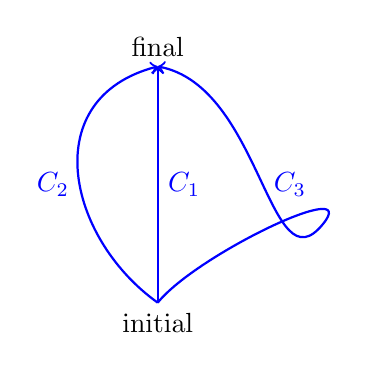
\begin{tikzpicture}[xscale=1.4]
		\draw[thick,->,blue] (0,0) node[below]{\textcolor{black}{initial}} -- (0,3) node[above]{\textcolor{black}{final}} node[midway,right]{$C_1$};
		\draw[thick,->,blue] (0,0) [out=135,in=200] to (0,3);
		\node[blue] at (-0.95,1.5) {$C_2$};
		\draw[thick,->,blue] (0,0) [out=60,in=60] to (1.5,1) [out=240,in=-15] to (0,3);
		\node[blue] at (1.2,1.5) {$C_3$};
		\end{tikzpicture}
	\end{center}
	\vspace{-20pt}
\end{wrapfigure}

work by gravitational force is path independent

for example, same work is done via path $C_1$, $C_2$ and $C_3$

so gravitational force is conservative, G.P.E. can be defined

as a consequence, gain or loss in G.P.E. only depends on the difference in initial and final position of the object

if there is no other conservative force acting on a body apart from gravitational force, it follows that change in total energy of an object equals the net work done by all forces excluding gravity





\subsubsection{conservation of energy}

\begin{ilight}
	\keypoint{the law of conservation of energy} states that energy cannot be created or destroyed, but can only transform from one form into another while the total amount is always constant  \index{conservation of energy}
\end{ilight}

in absence of any non-conservative force, sum of a body's kinetic energy and potential energies, or the total mechanical energy,  is constant, this is also a law of conservation


\example{For an object falling from rest due to gravity, if air resistance is negligible, what is its speed when it has fallen through a distance of $h$? }

\solc
\begin{equation*}
	\text{G.P.E loss} \,\,\, = \,\,\, \text{K.E gain} \RA mgh = \frac{1}{2}mv^2 \RA v=\sqrt{2gh} \teoe
\end{equation*}


\example{A marble is projected vertically upwards with an initial velocity $u$. The average resistive force acting is $f$. How do you determine the maximum height reached by the marble?}

\sol $\text{K.E. loss} \,\,\, = \,\,\, \text{G.P.E. gain} \,\,\, + \,\,\, \text{energy loss due to resistance}$
\begin{equation*}
	\frac{1}{2}mu^2 - 0 = mgH_\tmax + f H_\tmax \RA  H_\tmax = \frac{mu^2}{2(mg+f)}\teoe
\end{equation*}


\begin{wrapfigure}{R}{0.5\textwidth}
	\vspace{-20pt}
	\begin{center}
		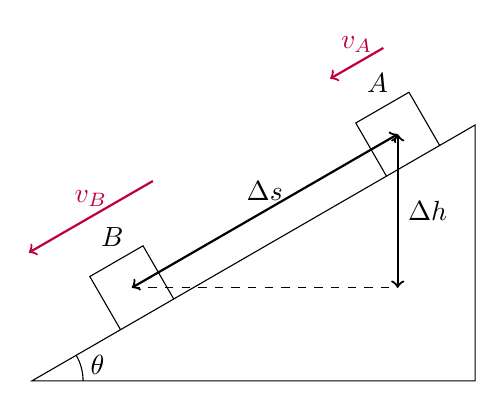
\begin{tikzpicture}[scale=1.3]
		\draw (0,0) -- (30:5) -- ++(0,-2.5) -- cycle;
		\draw (0.5,0) arc(0:30:0.5);
		\node at (0.64,0.16) {$\theta$};
		\draw (30:4) -- ++(120:.6) -- ++(30:.6) -- ++(-60:.6);
		\draw (30:1) -- ++(120:.6) -- ++(30:.6) -- ++(-60:.6);
		\draw[thick,<->] (30:4.3) ++ (120:0.3) -- ++ (30:-3) node[midway,above]{$\Delta s$};
		\draw[thick,purple,->] (30:4.6) ++ (120:1.1) -- ++ (30:-0.6) node[midway,above]{$v_A$} node[midway,below right]{\textcolor{black}{$A$}};
		\draw[thick,purple,->] (30:2.0) ++ (120:1.1) -- ++ (30:-1.4) node[midway,above]{$v_B$} node[midway,below right]{\textcolor{black}{$B$}};;
		\draw[thick,<->] (30:4.3) ++ (120:0.3) -- ++(0,-1.5) node[midway,right]{$\Delta h$};
		\draw[dashed] (30:1.3) ++ (120:0.3) -- ++(2.598,0);
		\end{tikzpicture}
	\end{center}
	\vspace{-25pt}
\end{wrapfigure}

\example{A box of mass $m$ slides down along a slope that is inclined at an angle $\theta$ to the horizontal. There is a constant friction $f$ acting on the box. When the box has moved through a distance of $\Delta s$ down the slope from $A$ to $B$, write down an equation relating its velocities $v_A$ and $v_B$ by applying the law of conservation of energy.}

\newpage

\solc\begin{eqnarray*}
		\text{work done against friction} &=& \text{change in total energy} \\
		-W_f &=& \Delta E_k + \Delta E_p \\
		-fs &=& \left( \frac{1}{2}mv_B^2 - \frac{1}{2}mv_A^2 \right) + \left( mgh_B - mgh_A \right) \\
		-fs &=& \left( \frac{1}{2}mv_B^2 - \frac{1}{2}mv_A^2 \right) - mg\Delta h \\
		v_B^2 &=& v_A^2 + 2g\Delta s \sin\theta - \frac{2fs}{m}
	\end{eqnarray*}
	
	or equivalently, we can write
	\begin{eqnarray*}
		\text{G.P.E loss} &=& \text{K.E gain} \,\,\, + \,\,\, \text{energy loss due to friction}\\
		mg\Delta h &=& \left( \frac{1}{2}mv_B^2 - \frac{1}{2}mv_A^2 \right) + fs \\
		v_B^2 &=& v_A^2 + 2g\Delta s \sin\theta - \frac{2fs}{m}
	\end{eqnarray*}
	
	note that the two alternative ways of thinking produce the same result \eoe


\begin{wrapfigure}{R}{0.5\textwidth}
	\vspace{-25pt}
	\begin{center}
		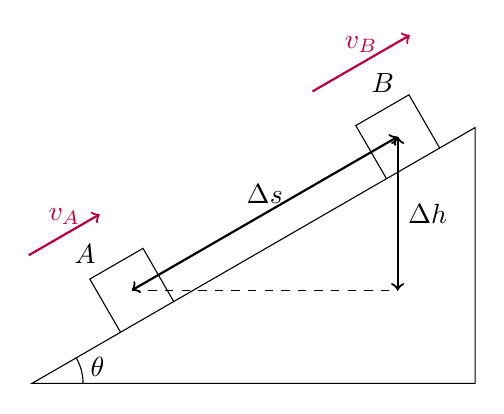
\begin{tikzpicture}[scale=1.3]
		\draw (0,0) -- (30:5) -- ++(0,-2.5) -- cycle;
		\draw (0.5,0) arc(0:30:0.5);
		\node at (0.64,0.16) {$\theta$};
		\draw (30:4) -- ++(120:.6) -- ++(30:.6) -- ++(-60:.6);
		\draw (30:1) -- ++(120:.6) -- ++(30:.6) -- ++(-60:.6);
		\draw[thick,<->] (30:4.3) ++ (120:0.3) -- ++ (30:-3) node[midway,above]{$\Delta s$};
		\draw[thick,purple,<-] (30:4.9) ++ (120:1.1) -- ++ (30:-1.1) node[midway,above]{$v_B$} node[midway,below right]{\textcolor{black}{$B$}};
		\draw[thick,purple,<-] (30:1.4) ++ (120:1.1) -- ++ (30:-0.8) node[midway,above]{$v_A$} node[midway,below right]{\textcolor{black}{$A$}};;
		\draw[thick,<->] (30:4.3) ++ (120:0.3) -- ++(0,-1.5) node[midway,right]{$\Delta h$};
		\draw[dashed] (30:1.3) ++ (120:0.3) -- ++(2.598,0);
		\end{tikzpicture}
	\end{center}
	\vspace{-15pt}
\end{wrapfigure}

\example{A slope is inclined at an angle $\theta$ to the horizontal. A box of mass $m$ is pushed up the slope with a constant force $F$ parallel to the slope, and the box experiences a constant frictional force $f$. When the box has moved through a distance of $\Delta s$ along the slope from $A$ to $B$, find an equation relating its velocities $v_A$ and $v_B$.}

\solc\begin{eqnarray*}
	\text{work by $F$ + work against friction} &=& \text{change in total energy} \\
	W_F-W_f &=& \Delta E_k + \Delta E_p \\
	Fs-fs &=& \left( \frac{1}{2}mv_B^2 - \frac{1}{2}mv_A^2 \right) + \left( mgh_B - mgh_A \right) \\
	Fs-fs &=& \left( \frac{1}{2}mv_B^2 - \frac{1}{2}mv_A^2 \right) + mg\Delta h \\
	v_B^2 &=& v_A^2 + \frac{2(F-f)s}{m} - 2g\Delta s \sin\theta 
\end{eqnarray*}

or equivalently, we can write
\begin{eqnarray*}
	\text{work by $F$} &=& \text{K.E gain} \,\,\, + \,\,\, \text{G.P.E gain} \,\,\, + \,\,\, \text{energy loss due to friction}\\
	Fs &=& \left( \frac{1}{2}mv_B^2 - \frac{1}{2}mv_A^2 \right) + mg\Delta h + fs \\
	v_B^2 &=& v_A^2 + \frac{2(F-f)s}{m} - 2g\Delta s \sin\theta 
\end{eqnarray*}

again the two approaches produce the same expression for final velocity \eoe

\begin{wrapfigure}{R}{0.4\textwidth}
	\vspace{-10pt}
	\begin{center}
		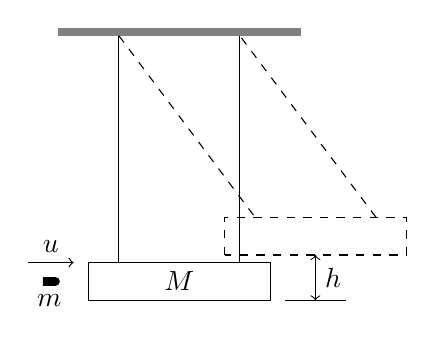
\begin{tikzpicture}[scale=.96]
		\draw[Gray,fill] (-0.8,0) rectangle (2.4,0.1);
		\draw (-0.4,-3.5) rectangle (2.0,-3);
		\node at (0.8,-3.25) {$M$};
		\draw[dashed] (1.4,-2.9) rectangle (3.8,-2.4);
		\draw (0,0) -- ++(0,-3) ++(1.6,0) -- ++(0,3);
		\draw [dashed] (0,0) -- ++(1.8,-2.4) ++(1.6,0) -- ++(-1.8,2.4);
		\draw[fill] (-1,-3.2) -- ++(0,-0.1) -- ++(0.16,0) node[midway, below]{$m$} arc (-90:90:0.05) -- ++ (-0.16,0);
		\draw[->] (-1.2,-3) -- ++ (0.6,0) node[midway,above]{$u$};
		\draw[<->] (2.6,-3.5) -- ++(0,0.6) node[midway,right]{$h$};
		\draw (2.2,-3.5) -- ++(0.8,0);
		\end{tikzpicture}
	\end{center}
	\vspace{-20pt}
\end{wrapfigure}


\example{A \emph{ballistic pendulum} is a device used to measure the speeds of fast-moving bullets. It consists of a large block of wood of mass $M$, suspended from two long light strings. A bullet of mass $m$ is fired into the block, and the block and bullet combination swings upward. If the centre of mass rises a vertical distance $h$, what is the initial speed $u$ of the bullet?}

\sol as bullet enters block, combined momentum is conserved:
\begin{equation*}
	mu = (M+m)v \RA v = \frac{mu}{M+m}
\end{equation*}

when the system swings upward, K.E. transforms into G.P.E. but total energy is conserved:
\begin{equation*}
\frac{1}{2}(M+m)v^2 = (M+g)gh \RA v = \sqrt{2gh}
\end{equation*}

putting the two equations together, we find: $ u = \left(1+\frac{M}{m}\right)\sqrt{2gh} $ \eoe








\subsection{power}

to describe how fast work is done, we introduce the notion of power

\begin{ilight}
	\keypoint{power} is defined as the work done per unit time: $\boxed{P = \frac{\Delta W}{\Delta t}}$  \index{power}
\end{ilight}

\cmt unit of power: $[P]  = \frac{[W]}{[t]} = \text{J s}^{-1} = \text{W (watt)}$

if one joule of work is done in one second, the power is one \keypoint{watt}

\cmt $P = \frac{\Delta W}{\Delta t}$ gives the \emph{average} power during in a period of time $\Delta t$

to find the \emph{instantaneous} power at a particular moment, we have
\begin{equation*}
P = \frac{\Delta W}{\Delta t} = \frac{F \Delta s}{\Delta t} \RA \boxed{P=Fv}
\end{equation*}

\example{There are 150 steps to the top of a tower, and the average height of each step is 25 cm. It takes a man of 72 kg two minutes to run up all the steps. What is his average power?}

\solc\begin{equation*}
	P = \frac{\Delta E_p}{\Delta t} = \frac{mg \Delta h}{\Delta t} = \frac{72\times9.81\times (150\times0.25)}{120} \RA P \approx 221 \text{ W} \teoe
\end{equation*}

\example{A turbine is used to generate electrical power from the wind. Given that the blades of the turbine sweep an area of 500 $\text{m}^2$, the density of air is	1.3 $\text{kg m}^{–3}$, and the wind speed is $10 \mps$. Assume no energy loss, find the power available from the wind.}

\eqyskip\solc\begin{equation*}
P = \frac{\Delta E_k}{\Delta t} = \frac{\frac{1}{2}\Delta m v^2}{\Delta t} = \frac{\frac{1}{2} \rho \Delta V v^2}{\Delta t} = \frac{\frac{1}{2} \rho A \Delta x v^2}{\Delta t} \RA P = \frac{1}{2} \rho A v^3 
\end{equation*}
\begin{equation*}
P = \frac{1}{2} \times 1.3 \times 500 \times 10^3 \approx 3.25 \times10^5 \text{ W}  \teoe
\end{equation*}


\example{A ship is cruising a a constant speed of $15 \mps$. The total resistive force acting is 9000 N. What is the output power of this ship?}

\sol constant speed so equilibrium between driving force and resistive force
\begin{equation*}
	P = F v = f v = 9000 \times 15 \RA P = 1.35 \times 10^5 \text{ W} \teoe
\end{equation*}


\example{A car of mass $800 kg$ accelerates from rest on a horizontal road. Suppose the engine provides a constant power of 24000 W, and the resistive force can be given by $f=16v$, where $v$ is the speed of the car in$\mps$. (a) What is the acceleration of the car when it is travelling at $15\mps$? (b) What happens to the car if it maintains this driving power?}

\sol equation of motion for the car is: $ F_\text{net} = F - f = ma \RA \frac{P}{v} - \alpha v = ma $

at $v=15\mps$: $\frac{24000}{15} - 16\times15 = 800a \RA a=1.7\mpss $

as car's velocity $v$ increases, driving force $F=\frac{P}{v}$ decreases, resistive force $f=\alpha v$ increases

so resultant force will decrease, the car will accelerate at a decreasing rate

eventually it reaches an equilibrium state where $F=f$, the car then travels at constant speed $v_t$
\begin{equation*}
F=f \RA \frac{P}{v_t} = \alpha v_t \RA \frac{24000}{v_t} = 16v_t \RA v_t \approx 38.7\mps \teoe
\end{equation*}



\subsection{efficiency}

efficiency of a system is given by: $\text{efficiency} = \frac{\text{useful energy output}}{\text{total energy input}} $, or $\boxed{\eta = \frac{W_\text{useful}}{W_\text{total}}}$

since $\Delta W = P \Delta t$, efficiency can also be evaluated in terms of power: $\boxed{\eta = \frac{P_\text{useful}}{P_\text{total}}}$ \index{efficiency}

\example{A water pumping system uses 3.0 kW of electrical power to raise water from a well. The pump lifts 1500 kg of water per minute through a vertical height of 8.0 m. What is the efficiency of the sysem?}

\solc\begin{equation*}
	\eta = \frac{\Delta E_p}{\Delta E_\text{in}} = \frac{\Delta m g h}{P_\text{in} \Delta t} = \frac{1500\times9.81\times8.0}{3000\times60} \RA \eta \approx 65.4 \% \teoe 
\end{equation*}

\example{Water flows into a turbine from a reservoir at a vertical distance of 70 m above. The water flows through the turbine at a rate of 2500 kg per minute. What is the output power of the turbine if it is 85\% efficient?}

\solc\begin{equation*}
P_\text{out} = \eta P_\text{in} = \eta \frac{\Delta E_p}{\Delta t} = \eta \frac{\Delta m g h}{\Delta t} = 85\% \times \frac{2500 \times 9.81 \times 70}{60} \RA P_\text{out} \approx 2.43 \times 10^4 \text{ W}
\end{equation*}


\ifthenelse{\includequestions=1}{



\subsection{end-of-chapter questions}

\subsubsection*{work}

\question{
	A trolley is pushed through a distance of 2.0 m with a force of $F=5.0$ N along a track. The trolley experiences a constant frictional force of 3.0 N. What is the work done by $F$?
}

\question{
	A child of mass 40 kg slides down a slope from a height of 2.0 m above the ground. The slide is of a length of 6.0 m. How much work is done by gravity?
}


\question{
	A dog pulls on a lead with a force of 20 N at an angle of 20$^\circ$ to the horizontal. As the dog moves 10 m along the playground, find the work done (a) by the dog, (b) by the person holding the lead.
}

\question{
	A satellite is orbiting around the earth in a circular orbit due to gravitational attraction. The gravitational force on the satellite always acts towards the centre of the earth. Does this force do any work?
}

\question{
	A fixed mass of gas at a pressure of $1.50 \times 10^5 \text{ Pa}$ and initial volume of $2.80 \times 10^{-4} \text{ m}^3$ is heated. The gas expands at a constant pressure to a final volume of $8.40 \times 10^{-4} \text{ m}^3$. Find the work done by the gas.
}

\subsubsection*{kinetic energy}

\question{Estimate the kinetic energy of a family car travelling at $40 \text{ km}$ per hour.}

\question{Object $B$ has double the mass and moves at twice the speed of object $A$. If the kinetic energy of object $A$ is $K$, what is the kinetic enery of $B$?}

\subsubsection*{gravitational potential energy}

\question{
	Estimate how much gravitational potential energy you gain when you get to the top of the highest building in your country?
}

\question{
	Four uniform bricks, each of mass $m$ and thickness $H$, are laid out on a table. In order to stack them on top of one another, how much work has to be done on the bricks?
}

\subsubsection*{work \& energy transformations}

\question{
	A stone is projected vertically upwards at a speed of $16 \mps$ from the ground. Air resistance is negligible. (a) What is the greatest height reached by the stone? (b) When the stone is at a height of 5.0 m, what is its speed? (c) If the stone is projected at an angle from the upward vertical with the same initial speed, what is its speed when it reaches a height ob 5.0 m?
}

\question{
	A hammer of mass 600 g hits a nail at a velocity of $10 \mps$. The nail is pushed into a plank by 3.0 mm. What is the average frictional force acting on the nail?
}

\question{A block of mass $m$ is pushed through a fixed distance along a horizontal frictionless surface by a constant force. Show that the final speed $v$ of the block has: $v\propto \frac{1}{\sqrt{m}}$}.

\question{
	A block of 3.0 kg is released from rest on a slope at an angle $\theta = \sin^{-1}\left(\frac{1}{5} \right)$ to the horizontal. As the block travels 6.0 m down the slope, it experiences a frictional force of 5.0 N. What is the final speed of the block?}

\question{
	A cyclist is travelling up a hill at a constant speed. The cyclist uses 640 J of energy to travel a distance of 25 m. If the total resistive force opposing the motion is 9.0 N, what is the increase in gravitational potential energy? To determine the increase in the height, what further information do you need?
}

\question{
	A pendulum of mass 120 g is released from a position that is 1.6 cm above its equilibrium position. (a) At what point in its motion is the kinetic energy of a pendulum bob at its maximum? (b) At what point is the gravitational potential energy at a maximum? (c) When the kinetic energy is half its greatest value, how much gravitational potential energy does it have?
}

\question{
	A particle of mass $m$ is initially at a height of $h$ above the ground. It is then released from rest. Just before hitting the ground, the particle gains a speed of $v$. What is the average resistive force acting on the particle during the fall?
}

\question{
	Men's pole vault (a athletic event in which a person jumps over a bar with the aid of a long, flexible pole) world record is about 6 m. Could this record be raised to, say, 10 m by using a longer pole? If not, why is it impossible?
}



\question{
	This question concerns the design of a roller coaster. One designer says each summit must be lower than the previous one. Another designer suggests that it does not matter what heights the summits are as long as the first one is the highest. What do you think?
}

\subsubsection*{conservative forces ($\star$)}

\question{
	Explain why gravitational force is conservative.
}

\question{
	A charged object is acted by an electric force in an electric field. State and explain whether the electric force is conservative.
}

\question{
	Is friction a conservative force? Explain your reasons.
}


\subsubsection*{power}
\question{
	A car engine exerts an average force of 400 N in moving the car 900 m in 200 s. What is the average power developed?
}

\question{
	During a human heart beat, about 20 g of blood is pushed into the main arteries. This blood is accelerated from a speed of $0.20 \mps$ to $0.35\mps$. For a heart pulsing at 75 beats per minute, what is the average power developed by the heart?
}

\question{
	Estimate your body power when you run upstairs at full speed.
}

\question{
	A truck of mass 2700 kg is travelling at a constant speed of $9.0\mps$ up a road that is inclined at 8.0$^\circ$ to the horizontal. Assume that the resistive forces are negligible. What is the useful power from the engine of the truck?
}

\question{Given that the forces resisting the motion of a racing car is proportional to the square of the car's speed. The car has an output power of 200 kW when travelling at a steady speed of $50\mps$. What output power is required to maintain a speed of $80\mps$?}

\question{
A car of mass 800 kg travels in a straight line up a slope. The total resistive force $f_R$ can be modelled by the equation: $f_R = kv^2$, where constant $k= \text{5.0 kg m}^{-1}$ and $v$ is the car's speed. When the car travels at a steady speed of $10\mps$, the engine exerts a force of 2.1 kN up the slope. (a) Find the component of the car's weight down the slope, and hence find the angle that the slope makes with the horizontal. (b) Find the power output from the engine. (c) If the car then travels onto a horizontal road. The engine's output power is unchanged and the resistive force obeys the same model as before. Find the acceleration of the car when its speed is $15\mps$. (d) The car eventually reaches a constant speed on the horizontal road. Find this terminal speed.
}

\subsubsection*{efficiency}
\question{
	An electric motor is used to lift a mass. When operating at full power, the current in the motor is 2.0 A and the voltage is 5.0 V. If the motor is 50\% efficient, what is the time take to lift a mass of 400 g through a height of 2.5 m?
}

\question{
	A turbine at a hydroelectric power station is designed to drive a generator to produce electrical energy. The water falls through a vertical distance of 8.0 m at a rate of 150 kg per second as it passes through the turbine. The generator supplies a current of 24 A at a voltage of 220 V. What is the efficiency of the turbine system?
}

\question{When power to the grid is not required during the night, 200 MW of electrical power is used to pump water from a reservoir up to a lake 300 m higher. The pumping system operates at an efficiency of 90\%. What mass of water can be pumped to the lake in three hours?}

\question{Given that the petrol engine for a real car is 25\% efficient. The fuel consumption for the engine is 16 litres per hour, and the energy density of the fuel is 44 MJ per litre. What is the power output from the engine?}

\question{A bow shoots an arrow of mass 150 g vertically upwards with an initial speed of $30 \mps$. The potential energy stored in the bow before release is 200 J. The arrow reaches a height of 30 m above the point of release. (a) What is the energy loss just after the arrow is released? (b) What is the efficiency of the bow for converting its potential energy into useful kinetic energy? (c) What is the energy loss due to air resistance? (d) What is the average force due to air resistance?}

}{}